\section{Propiedades Físicas}

\begin{frame}{Definiendo los Cerámicos: Más que Alfarería}
	\begin{block}{Definición Central}
		Sólidos inorgánicos, no metálicos, típicamente preparados mediante
		calentamiento y posterior enfriamiento.
	\end{block}

	\begin{itemize}
		\item Esta simple definición oculta una vasta complejidad en su química,
			estructura y propiedades.
		\item La clave para entender los cerámicos reside en sus enlaces
			interatómicos.
	\end{itemize}
\end{frame}

\begin{frame}{El Corazón de los Cerámicos: Enlaces Interatómicos}
	\begin{columns}[T]
		\begin{column}{0.5\textwidth}
			\begin{alertblock}{Enlaces Cerámicos Primarios}
				Caracterizados por fuertes \textbf{enlaces iónicos y/o covalentes}.
				\begin{itemize}
					\item Alta energía de enlace.
					\item Fuerzas intensas, a menudo direccionales.
				\end{itemize}
			\end{alertblock}
		\end{column}
		\begin{column}{0.5\textwidth}
			\begin{exampleblock}{En Contraste}
				\begin{itemize}
					\item \textbf{Metálico}: Mar de electrones, no direccional.
					\item \textbf{Polimérico}: Fuerzas débiles de van der Waals.
				\end{itemize}
			\end{exampleblock}
		\end{column}
	\end{columns}

	\begin{block}{Consecuencias del Enlace Fuerte}
		Altos puntos de fusión, dureza significativa y excelente estabilidad química.
	\end{block}
\end{frame}

\begin{frame}{Estructura Cristalina: Orden vs. Caos}
	\begin{columns}[T] % El entorno de columnas ya está creado

		% --- Columna Izquierda: Cristalino ---
		\begin{column}{0.5\textwidth}
			\begin{block}{Cristalinos (Ordenados)}
				Estructura atómica repetitiva y de largo alcance.

				% --- Comando para insertar la imagen ---
				\begin{figure}
					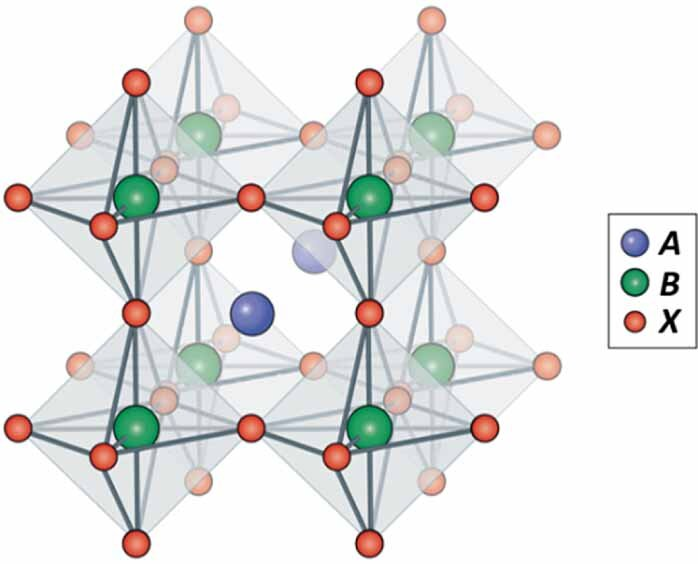
\includegraphics[width=0.7\linewidth]{../figures/perovskite-crystal-structure-CaTiO3-ABX3.jpg}
					\caption{Ej: Estructura de Perovskita (\ce{CaTiO3}) \cite{ng_group-iii-nitride_2021}}
				\end{figure}

			\end{block}
		\end{column}

		% --- Columna Derecha: Amorfo ---
		\begin{column}{0.5\textwidth}
			\begin{block}{Amorfos (Desordenados)}
				Estructura atómica sin un orden a largo plazo.

				% --- Comando para insertar la imagen ---
				\begin{figure}
					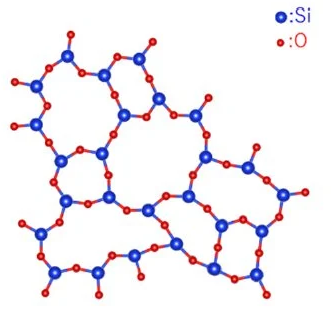
\includegraphics[width=0.6\linewidth]{../figures/Schematic-of-silica-molecule.png}
					\caption{Ej: Red de sílice vítrea (\ce{SiO2}) \cite{kohara_relationship_2011}}
				\end{figure}

			\end{block}
		\end{column}

	\end{columns}
\end{frame}

\begin{frame}{Estructura-Propiedad I: Comportamiento Mecánico}
	\begin{alertblock}{El Problema de la Fragilidad}
		Alta resistencia a la compresión, pero baja resistencia a la tracción y
		tenacidad a la fractura ($K_{IC}$).
	\end{alertblock}

	\begin{itemize}
		\item \textbf{Teoría de la Fractura Frágil de Griffith}: Defectos
			nanoscópicos preexistentes (\textit{grietas de Griffith}) actúan como
			concentradores de esfuerzo, llevando a una falla catastrófica bajo
			tensión.
			\pause
		\item \textbf{Razón Fundamental}: Los enlaces fuertes y direccionales
			resisten el movimiento de dislocaciones. La energía se libera mediante la
			propagación de grietas, no por deformación plástica.
	\end{itemize}
\end{frame}

\begin{frame}{Estructura-Propiedad II: Propiedades Térmicas y Eléctricas}
	\begin{columns}[T]
		\begin{column}{0.5\textwidth}
			\begin{block}{Propiedades Térmicas}
				\begin{itemize}
					\item Generalmente baja conductividad térmica debido a la
						\textbf{dispersión de fonones} efectiva en redes cristalinas
						complejas.
					\item Alta estabilidad térmica debido a la alta energía de enlace.
				\end{itemize}
			\end{block}
		\end{column}
		\begin{column}{0.5\textwidth}
			\begin{block}{Propiedades Eléctricas}
				\begin{itemize}
					\item Excelentes aislantes. Explicado por la \textbf{teoría de
						bandas}: una gran banda prohibida ($E_g$) previene la excitación de
						electrones.
					\item Los defectos/dopaje pueden crear estados en la banda prohibida,
						conduciendo a un comportamiento semiconductor.
				\end{itemize}
			\end{block}
		\end{column}
	\end{columns}
\end{frame}

\begin{frame}{Clasificación: Una Historia de Dos Cerámicos}
	\begin{block}{Cerámicos Tradicionales}
		\begin{itemize}
			\item Productos a base de arcilla (alfarería, ladrillo, porcelana).
			\item Compuestos de materias primas naturales no refinadas.
		\end{itemize}
	\end{block}
	\vspace{1cm}
	\begin{alertblock}{Cerámicos Avanzados / Técnicos}
		\begin{itemize}
			\item Materiales sintéticos de alta pureza diseñados para un rendimiento
				funcional o estructural específico.
			\item Ejemplos: \ce{Al2O3}, \ce{Si3N4}, \ce{BaTiO3}.
		\end{itemize}
	\end{alertblock}
\end{frame}
